\documentclass{beamer}
\usepackage{graphicx}
\usepackage{hyperref}
\usepackage{pdfpages}
\usepackage{amsmath}
\usepackage{amsfonts}
\usepackage{amssymb}
\usepackage{array}
\hypersetup{colorlinks=true}
\newcommand{\R}{\mathbb{R}}
\begin{document}
\begin{frame}
  \begin{center}
    t-Distributed Stochastic Embedding \\
    Sigma Seminar, UConn \\
    October 4, 2019
  \end{center}
\end{frame}
\begin{frame}
  \frametitle{The Problem}
  
    Given a data set in a high dimensional space, about which little is known {\it a priori},
    find structure that can be used for further study.
  
\end{frame}
\begin{frame}
  \frametitle{Example}
  \begin{enumerate}
  \item A single-cell RNA expression experiment produces a $10000\times 30000$ matrix.
  \item Each row of the matrix corresponds to a cell and the $30000$ numbers represent the ``state'' of the cell.
  \item One would like to identify classes of cells that are ``similar'' and then do further analysis to characterize what makes them so.
  \item How can one extract these similar classes from the data?
  \end{enumerate}
\end{frame}

\begin{frame}
  \frametitle{A strategy}
  Find a way to embed the data in $2$ (or $3$) dimensions while preserving as much of the structre as possible.
  If the two dimensional representation captures enough of the structure in the high dimensional space, then one can see patterns in the data,
  or use low-dimensional tools to study the data.

\end{frame}
\begin{frame}
  \frametitle{Principal Component Analysis}
\begin{itemize}
\item   Let $X$ be a $k\times N$ matrix whose rows $x_{j}$ correspond to samples and whose coordinates in $\R^{N}$ are particular measurements.  Assume that the matrix is ``centered'' so that the mean of every column is zero.

\item  The goal of PCA is to find a linear combination of the measurements that does the best job of separating the observations.

\item   If $w$ is a $N\times 1$ unit vector,  then $Xw$ gives the value of a new linear combination of measurements for each data point. The
  dot product $w^tX^tXw$ then measures the variance of this new measurement.  So our goal is to maximize $\|w^{t}X^{t}Xw\|$,
  and linear algebra tells us this is achieved when $w$ is the eigenvector of $X^{t}X$ with maximum eigenvalue.

\item   More generally projecting $X$ into the span of the top $k$ eigenvectors captures the most significant linear variations in the data.
\end{itemize}
\end{frame}
\begin{frame}
  \begin{center}
  \begin{tabular}{cc}
  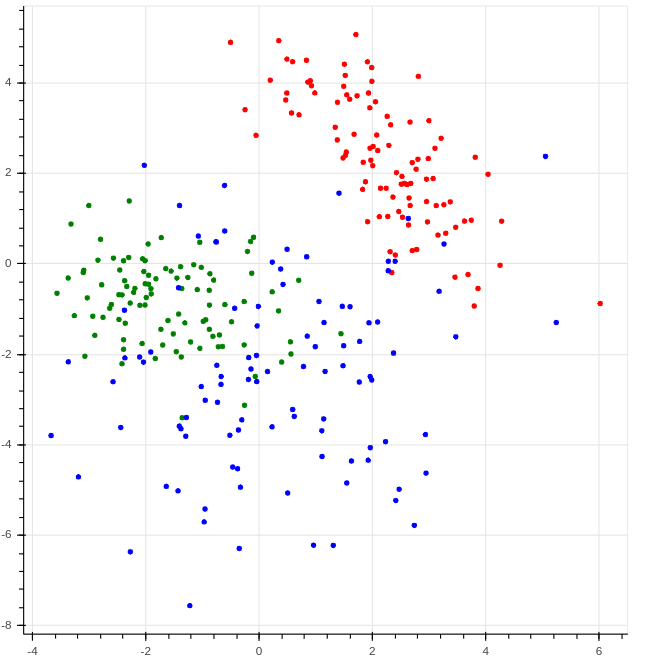
\includegraphics[width=2in]{pca_data.png} &
  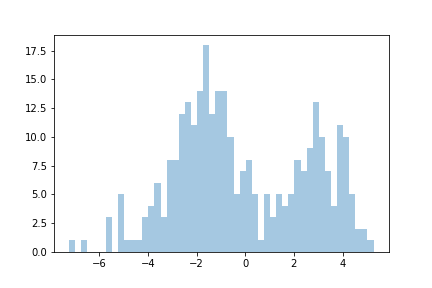
\includegraphics[width=2in]{pca_hist.png}\cr
  {\small Original Data} & {\small Projection onto Principal Direction} \cr
  \end{tabular}

  PCA can only detect variation in the features along linear subspaces.
\end{center}
\end{frame}
\begin{frame}
  \frametitle{More general methods}

  Given a $k\times N$ data matrix $X$, a general dimension reduction algorithm is derived from:
  
  \begin{enumerate}
  \item   a symmetric 'similarity matrix' $P$ whose   entries $p_{ij}$ measure the similarity of the points $x_i$ and $x_j$.  This could be:

    \begin{itemize}
    \item the Euclidean distance between   $x_i$ and $x_j$
    \item some weighted version of the Euclidean distance
    \item some domain-specific measure of similarity
    \end{itemize}

  \item A similarity function $Q$ that compares points $y_i$ and $y_j$ in $\mathbb{R}^{2}$ that correspond to the $x_i$. 
  \item A comparison between $P$ and $Q$ that measures the fidelity of the correspondence between $x_i$ and $y_i$.
  \end{enumerate}
  One tries to find points $Y$ in $\mathbb{R}^{2}$ in a way that minimizes the ``difference'' between $P$ and $Q$.
\end{frame}
\begin{frame}
  \frametitle{The curse of dimensionality}
\begin{itemize}
\item  The biggest obstacle to finding a good embedding of high dimensional data in a low dimensional space is that it's impossible.

\item  There are many ways in which high dimensional space is ``different'' than our intuition.
\end{itemize}

\end{frame}
\begin{frame}
  \frametitle{The curse of dimensionality}

\begin{itemize}
\item  The unit hypersphere in dimension $n$ (unit ball in $\ell^{2}$-norm) has volume $\pi^{n/2}/n\Gamma(n/2)$

\item  The enclosing cube (the unit ball in the $\ell^{\infty}$-norm)  has volume $2^n$.

\item Comparing:
  $$
  \lim_{n\to\infty}\frac{\pi^{n/2}}{n2^{n}\Gamma(n/2)}= 0
  $$
\item
  Therefore the sphere becomes an ever smaller fraction of the cube and so bounding the coordinates of a point becomes a much weaker condition than
  bounding the $L^2$-norm.

\end{itemize}
  Among many other problems, this causes ``crowding'' in dimensionality reduction -- trying to fit too many points into small regions in $\mathbb{R}^{2}$.
\end{frame}

\begin{frame}
  \frametitle{t-SNE: An example}
\begin{block}{}
  The Fashion-MNIST data set is a collection $60k$ images of items of clothing (shirts, pants, dresses, purses, jackets, shoes).  Each image is
  a $28\times 28$ matrix real valued where the entries are the ``darkness'' of that point, from $0$ being white to $1$ being black.
\end{block}
\begin{block}{}
So we may view each image as a vector in $\R^{784}$.
\end{block}
\begin{block}{}
  Without knowing anything about the images, what structure can we recover?
\end{block}
\end{frame}
\begin{frame}
  \frametitle{Example}
  \begin{center}
    \href{http://tsne-fashion.herokuapp.com}{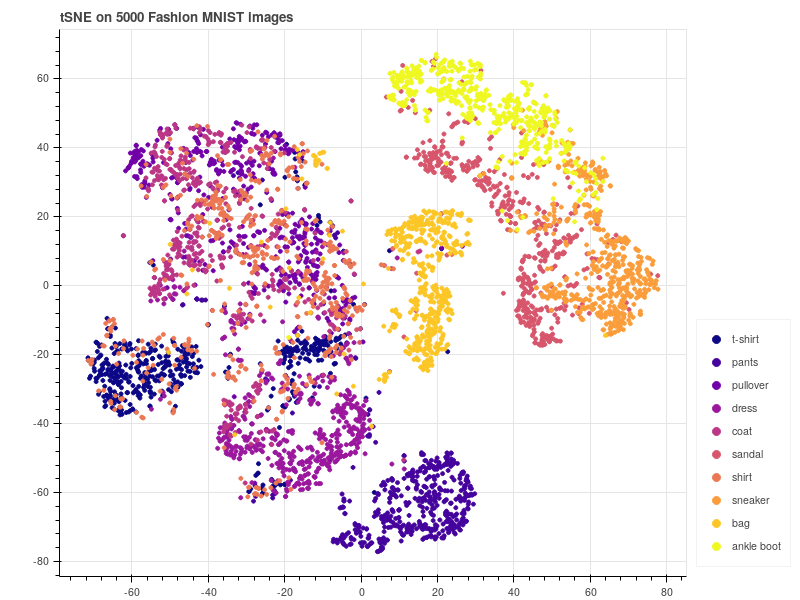
\includegraphics[width=3in]{tsne_fashion.png}}
  \end{center}
\end{frame}
\begin{frame}
  \frametitle{Ingredients of t-SNE}
  Note: Before applying tSNE, one projects the data into a lower dimensional space (say, 30 or 50 dimensions) using PCA. This focuses on the most significant
  variation.
  \bigskip\noindent
  
  The main ingredients of the t-SNE algorithm are:
  \begin{itemize}
  \item A gaussian-weighted similarity function in the high dimensional space.
  \item A t-distributed (Cauchy-distributed) similarity function in $\R^{2}$
  \item The Kullback-Leibler divergence as a measure of fidelity between the two distributions
  \item Gradient descent as an optimization process
  \end{itemize}
\end{frame}
\begin{frame}
  \frametitle{Gaussian similarity and perplexity}
  Given a point $x_i$ in the original data set, let
  $$
  p_{j|i}(\sigma)=\frac{e^{-\|x_j-x_i\|^2/2\sigma^2}}{Z_i(\sigma)}
  $$
  where $Z_i(\sigma)=\sum_{k\not=i}e^{-\|x_k-x_i\|^2/2\sigma^2}$.
  \bigskip\noindent

  In some sense, $p_{j|i}(\sigma)$ measures the chance that point $x_j$ would be selected as a neighbor for point $x_i$.  We set $p_{i|i}=0$.
  \bigskip\noindent

  The $\sigma$ parameter controls the ``reach'' of the point $x_i$.
  
\end{frame}
\begin{frame}
  \frametitle{Perplexity}
  If $P=\{p_i\}$ is a discrete probability distribution, the Shannon entropy $H(P)$ of $P$ is defined by
  $$
  H(P)=-\sum_{i} p_i\log_2 p_i.
  $$
  Entropy measures the uncertainty of the distribution; it is maximum when the $p_i$ are all equal, and gets smaller if certain events are more likely than others. In some ideal sense, entropy is the number of bits needed to encode the output of the process.
  \bigskip\noindent

  The perplexity is defined to be $2^{H(P)}$.  Since entropy measures the number of bits necessary to encode the process, perplexity is (in some sense) the
  effective number of states of the process.
\end{frame}
\begin{frame}
  \frametitle{Choosing $\sigma_i$ for tSNE}
  The tSNE algorithm chooses the $\sigma_i$ so that the perplexities of $p_{j|i}(\sigma_i)$ are all the same (and equal to some pre-set parameter).
  \bigskip\noindent

  In the original t-SNE paper, the author suggests thinking of this parameter as choosing the effective number of neighbors for each point in the
  dataset.

  The algorithm uses a binary search for each point $x_i$ to adjust $\sigma_i$ until the perplexity is set to the preassigned value.
\end{frame}
\begin{frame}
  \frametitle{The high-dimensional similarity}
  The distance $P_{j|i}$ constructed above is not symmetric.  To rectify this, the t-SNE algorithm symmetrizes it.
\bigskip\noindent

  One way to think of this is to consider the fact that the relation ``$p$ is one of the $k$ points closest to $q$'' is not symmetric.
  Making $P_{j|i}$ symmetric is an analytic way of creating the symmetric relation ``$p$ is one of the $k$ points closest to $q$, or vice versa.''
  \bigskip\noindent

  This brings outlier points into fuller consideration when constructing the low-dimensional map.
\end{frame}

\begin{frame}
  \frametitle{The low-dimensional similarity}
  The t-SNE algorithm uses a ``Cauchy Distribution'' to measure similarity in the low-dimensional space. Set
  $$
  q_{ij}=\frac{(1+\|y_i-y_j\|^2)^{-1}}{K}
  $$
  where $K=\sum_{k\not=l}(1+\|y_k-y_l\|^2)^{-1}$.
  \bigskip\noindent

  This function decays much more slowly as the distance between the points grows than the gaussian does.  In some sense this means
  the algorithm allows more ``spread'' in the low dimensional space than the high dimensional one to make up for the lack of ``room''
  in the low-dimensional space.
\end{frame}
\begin{frame}
  \frametitle{t-distribution vs gaussian comparison}
\begin{center}
  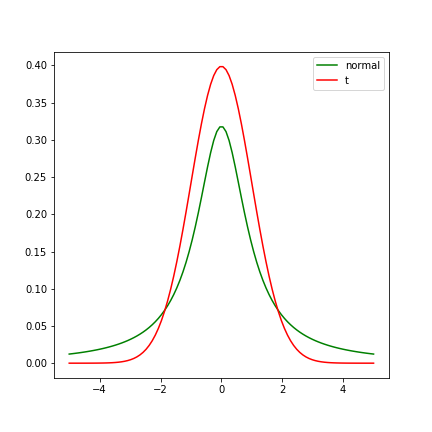
\includegraphics[width=2in]{norm_t.png}
\end{center}
\end{frame}
\begin{frame}
  \frametitle{Comparing the high and low-dimensional similarity}
  The metric tSNE uses to compare the two similarity measures is called the Kullback-Leibler divergence or the {\it relative entropy.}
  \bigskip\noindent
  
  Given two (discrete) probability
  measures $p$ and $q$, the KL divergence is defined as
  $$
  KL(p||q)=-\sum_{i} p_i\log\frac{q_i}{p_i}
  $$

  Note that this is not symmetric.
\end{frame}
\begin{frame}
  \frametitle{KL divergence}

  KL divergence measures the extra information required to describe data originating from the distribution $p$ if we use the ``wrong'' model $q$
  to describe it.
  \bigskip\noindent

  While perhaps not particularly quantitative, one way to think of this is that the KL divergence measures how surprised we should be if
  the low-dimensional picture says that two points are close, but they are in fact not close in the high dimensional space.
  \bigskip\noindent

  In this sense, minimizing the KL divergence means that the low dimensional picture does the best job capturing the relationships in the high
  dimensional space

  \bigskip\noindent

  Unfortunately, this minimization problem may have multiple local minima.
\end{frame}
\begin{frame}
  \frametitle{Gradient Descent}
  The problem of finding local minima for the KL divergence can be attacked by gradient descent. If $f:\mathbb{R}^{n}\to\mathbb{R}$
  is a differentiable function, then we know from multivariate calculus that the gradient
  $$
  \nabla f = \sum_{i}\frac{\partial f}{\partial x_i}\mathbf{e}_{i}
  $$
  points in the direction in which $f$ increases most rapidly, and its negative points in the direction in which it decreases most rapidly.
  \bigskip\noindent

  So we can choose a small step size $\delta$ and iteratively compute
  $$
  x^{(j+1)}=x^{(j)}-\delta\nabla f(x^{(j)})
  $$
  until we reach a point where the gradient is small enough that $x^{(j+1)}$  and $x^{(j)}$ are almost the same.
\end{frame}
\begin{frame}
  \frametitle{The tSNE gradient}
  A careful computation using the chain rule gives a formula for the gradient of the KL divergence between $P$ and $Q$. Here $P$ is fixed and we are varying
  the points $y$ in the low dimensional space, and hence varying $Q$ and then $C=KL(P||Q)$.
  $$
  \frac{\partial C}{\partial y_i} =
  4\sum_{i,j} (p_{ij}-q_{ij}) (y_i-y_j) (1+\|y_i-y_j\|^2)^{-1}
  $$
\end{frame}
\begin{frame}
\frametitle{The gradient (cont'd)}

  The gradient's dependence on the relative position of the points $x_i$ and $x_j$ in the high dimensional space, and $y_i$ and $y_j$ in the low space,
  is shown in this graph, taken from \href{https://lvdmaaten.github.io/publications/papers/JMLR\_2008.pdf}{van der Maaten's and Hinton's original tSNE paper}.
\begin{center}
  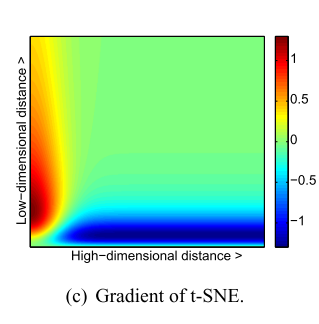
\includegraphics[width=2in]{tsneGradient.png}

There are both repulsive and attractive forces at work.
\end{center}
\end{frame}
\begin{frame}
  \frametitle{Some remarks on implementation}
  tSNE is an $O(N^2)$ algorithm.  To make it more practical there are some modifications that yield $O(N\log N)$.
  \bigskip\noindent

  First, one can optimize the computation of the $P$ matrix by only computing the $p_{j|i}$ for, say, the $k$ closest points to $x_i$.
  One can efficiently find the $k$ closest points using, for example, {\it vantage points trees.}  These are a data structure specifically
  designed for this purpose.
  \bigskip\noindent

  This makes $P$ sparse -- there are only a few non-zero entries in each row.
\end{frame}
\begin{frame}
  \frametitle{Optimization}
For the gradient descent phase, one can use a variant of the Barnes-Hut technique originally developed for computing orbital mechanics of large systems. In this approach you split the gradient into a repulsive and an attractive part:
  $$
  \frac{\partial C}{\partial y_i} = 4 (\sum_{j\not=i}p_{ij}q_{ij}Z(y_i-y_j)-\sum_{j\not=i}q_{ij}^2Z(y_i-y_j))
  $$
  where $q_{ij}Z=(1+\|y_i-y_j\|^2)^{-1}$ takes constant time to compute.
  \bigskip\noindent

  The first sum requires adding terms corresponding to non-zero entries in $p_{ij}$, which is sparse, so this takes time $O(N)$.
 \end{frame}
 \begin{frame}
   \frametitle{Optimization}
   For the second term, one applies the Barnes-Hut algorithm originally used for computations in orbital mechanics of complex systems.  The idea is
   that if a bunch of points $y_i$ are close together, one may approximate their contribution to the force by replacing them with their
   center of mass.
   \bigskip\noindent

   The BH algorithm partitions space into cubes that are small enough that the center of mass of the points in each cube are a good summary of the data.
 \end{frame}
 \begin{frame}
   \frametitle{Limitations}
   \begin{itemize}
   \item Gradient descent is initialized with random data, and since there are multiple local minima of the objective, different starting positions yield different results.  Running the algorithm several times may give ``better'' or ``worse'' visualizations.
   \item There is no ``map'' from the higher dimensional space to the lower one; and as a result you can't compute a visualization and then add new data and see where it lies.  (There is a parametric version of tSNE that addresses this problem.)
   \item Similarly, since there's no map, it isn't clear how to interpret the result of tSNE beyond ``what you see is what you get.''  You can't make inferences about the original data from the low dimensional picture.
   \end{itemize}
 \end{frame}
 \begin{frame}
   \frametitle{References}

   Hinton and van der Maaten, Visualizing High Dimensional Data with t-SNE, Journal of Machine Learning Research, 2008
   \bigskip\noindent

   van der Maaten, Accelerating t-SNE using Tree-Based Algorithms, Journal of Machine Learning Reserach, 2014.
 \end{frame}
 
  
\end{document}
%%% Local Variables:
%%% mode: latex
%%% TeX-master: t
%%% End:
